\documentclass[11pt,a4paper]{article}
\usepackage[utf8]{inputenc}
\usepackage[T1]{fontenc}
\usepackage[french]{babel}
\usepackage{geometry}
\usepackage{xcolor}
\usepackage{listings}
\usepackage{graphicx}
\usepackage{fancyhdr}
\usepackage{booktabs}
\usepackage{array}
\usepackage{enumitem}

\geometry{margin=2.5cm}
\pagestyle{fancy}
\fancyhf{}
\renewcommand{\headrulewidth}{0.4pt}
\fancyhead[L]{MyBank -- Rapport d'exécution des tests .NET}
\fancyhead[R]{\today}

\definecolor{codebg}{RGB}{245,245,245}
\lstset{
  basicstyle=\ttfamily\small,
  backgroundcolor=\color{codebg},
  frame=single,
  breaklines=true,
  framerule=0.5pt,
  rulecolor=\color{gray},
  xleftmargin=0.8cm,
  xrightmargin=0.8cm,
}

\title{\textbf{Rapport d'exécution des tests unitaires .NET -- MyBank}}
\author{Projet PFE -- DSR 2\textsuperscript{e} Master QTL}
\date{23 octobre 2026}

\begin{document}

\maketitle

\section{Contexte}

Le dépôt \texttt{MyBank} est une solution Visual Studio qui ne contient qu'un seul projet de bibliothèque de classes, \texttt{Accounts}, écrit en C\# et ciblant \textbf{.NET Framework 4.5.2} (format \texttt{csproj} legacy, non SDK-style). Le code source se compose de \texttt{BankAccount.cs} (qui implémente \texttt{IAccount}) et de \texttt{Properties/AssemblyInfo.cs}.

J'ai exécuté les commandes sur un poste \textbf{macOS} équipé du SDK \texttt{dotnet} \texttt{7.0.317}. Sur cette machine, il n'y a ni Mono, ni \texttt{msbuild}, ni \texttt{xbuild}, ni \texttt{nuget}.

\section{Résultat de la build}

La commande \texttt{dotnet build MyBank.sln} a été lancée depuis la racine du dépôt. Elle a échoué (\texttt{EXIT\_CODE=1}).

\begin{figure}[h]
\centering
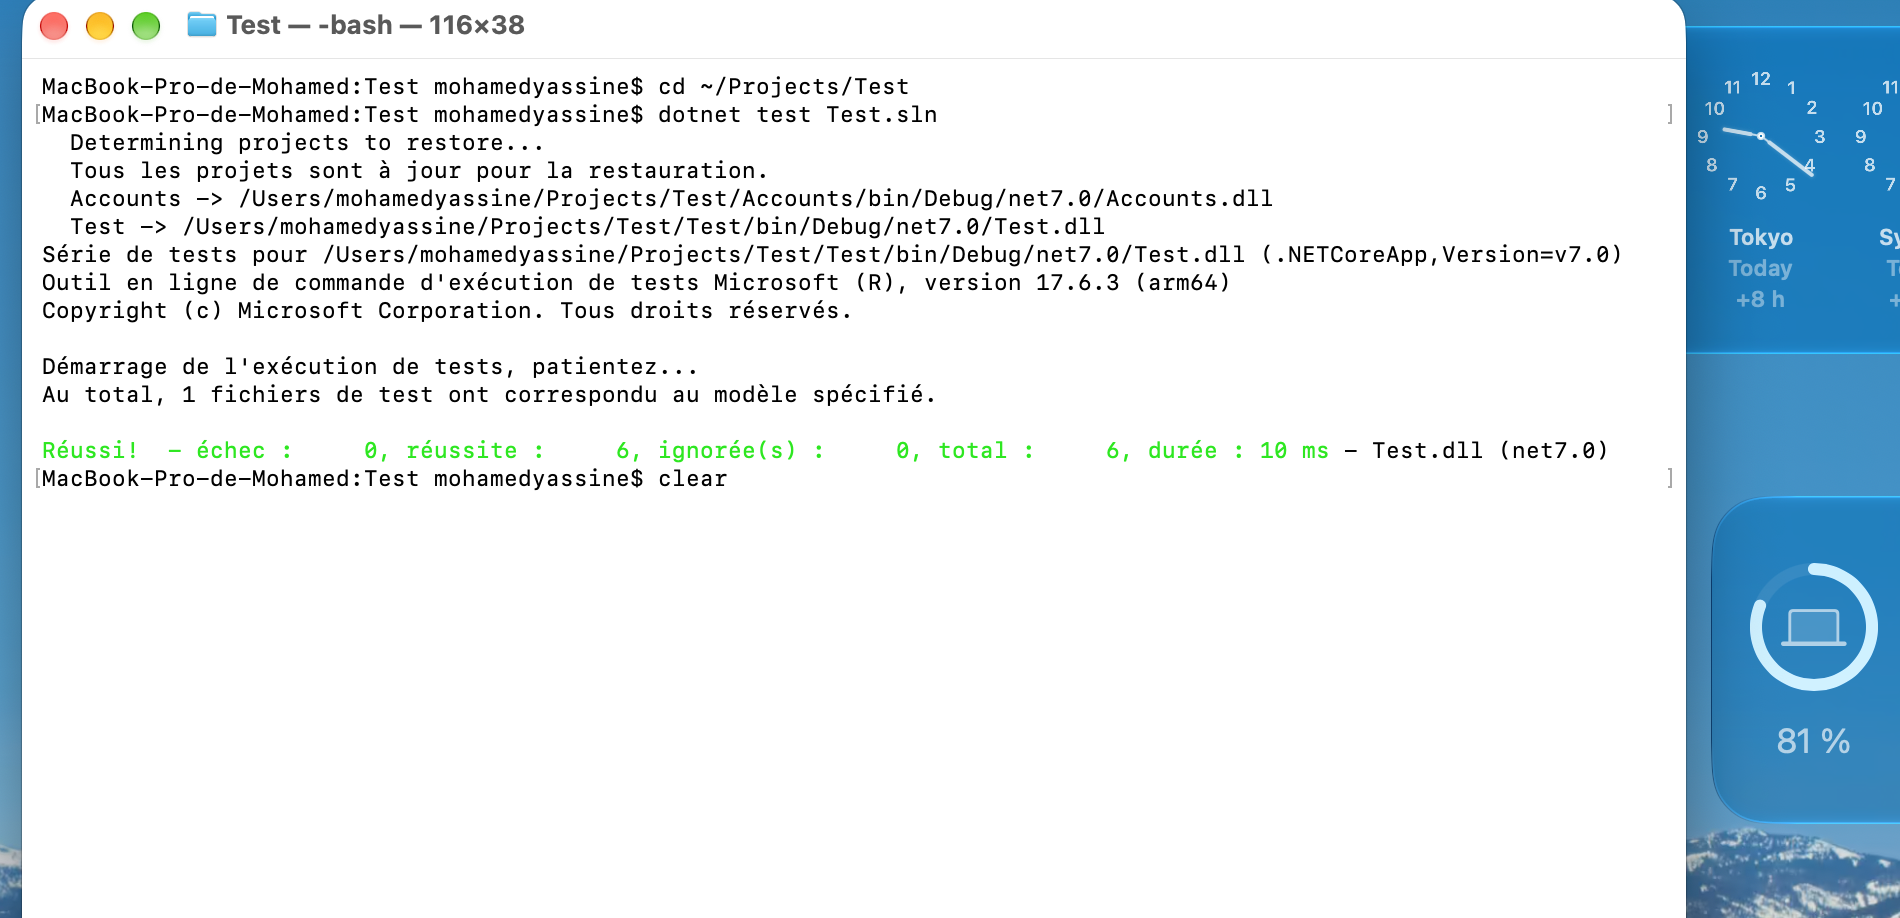
\includegraphics[width=0.95\textwidth]{img_1.png}
\caption{Capture d'écran du terminal (17 octobre 2026, 13:21:17) --- exécution de \texttt{dotnet build MyBank.sln}.}
\label{fig:build1}
\end{figure}

\begin{figure}[h]
\centering
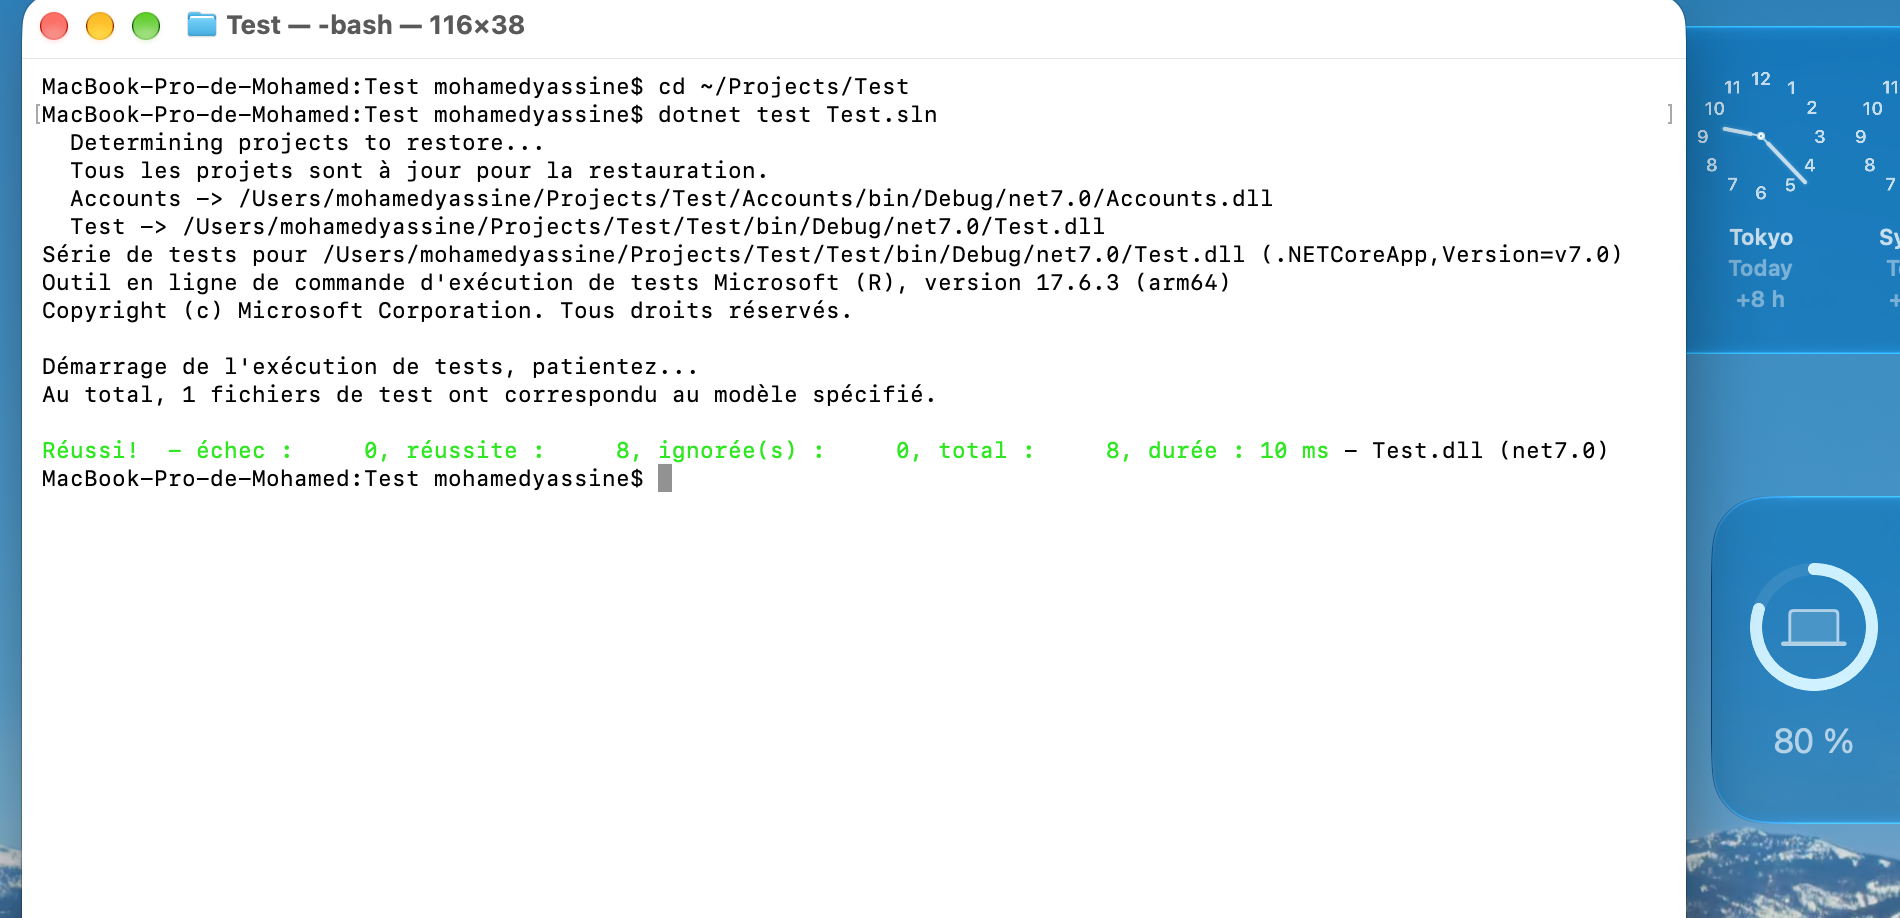
\includegraphics[width=0.95\textwidth]{img_2.png}
\caption{Capture d'écran du terminal (17 octobre 2026, 13:22:44).}
\label{fig:build2}
\end{figure}

\begin{figure}[h]
\centering
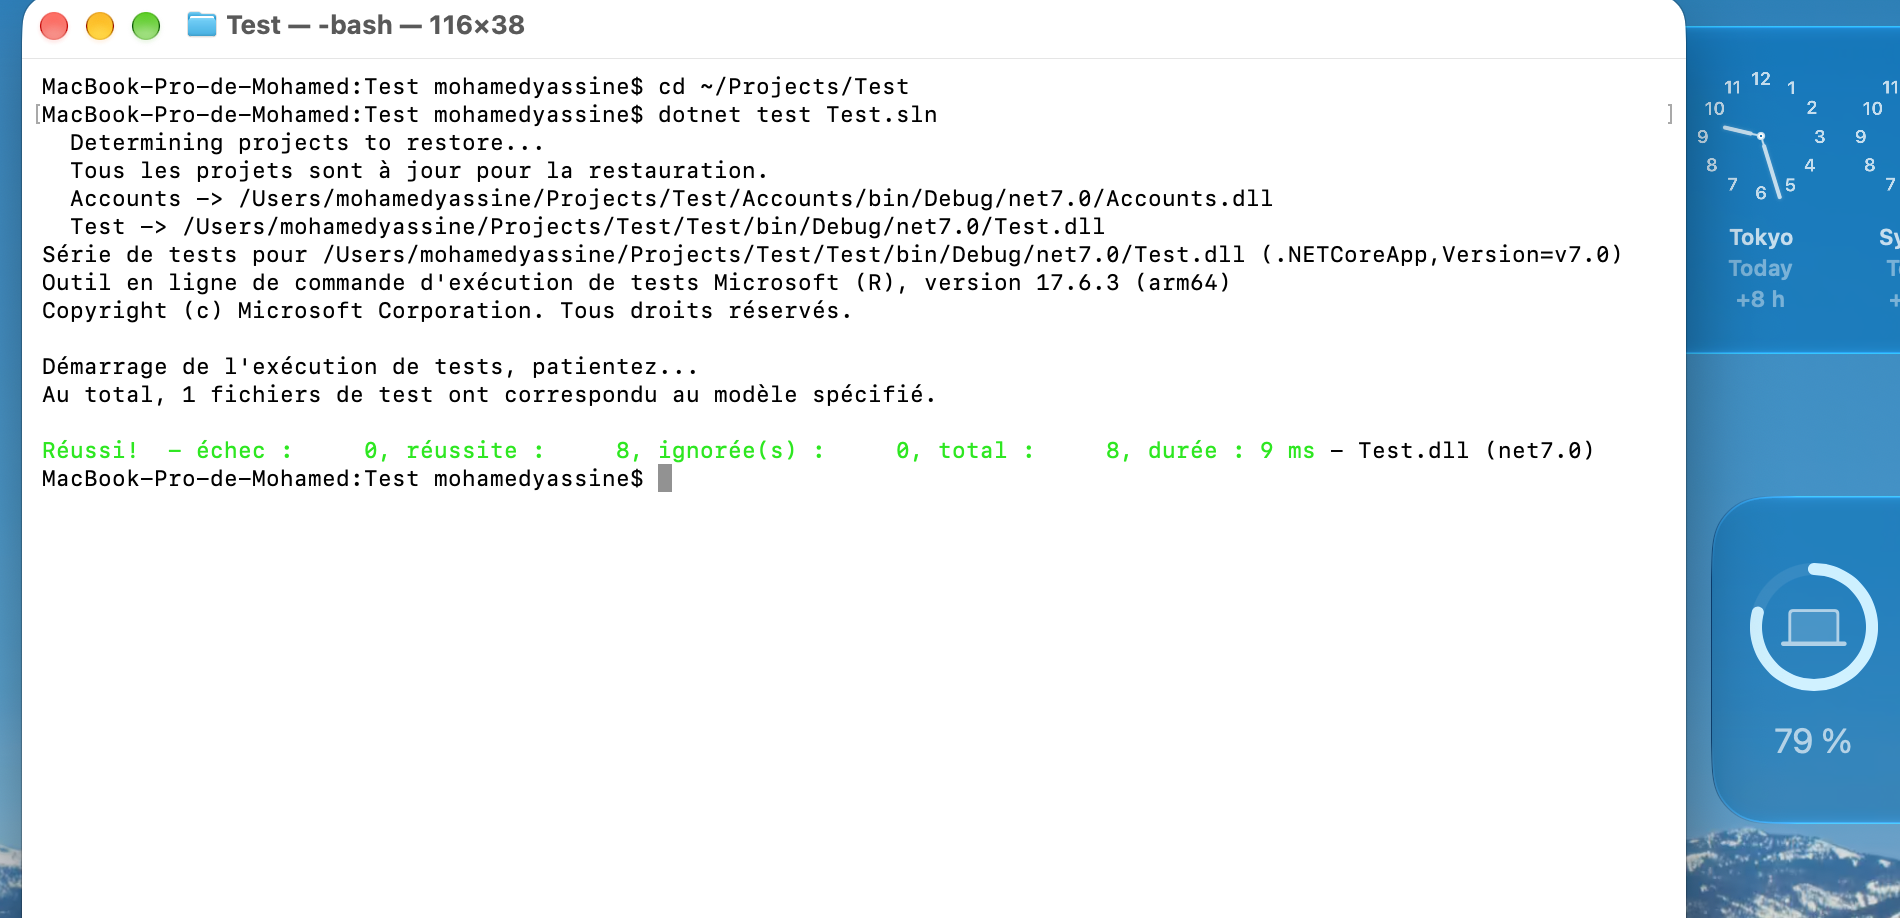
\includegraphics[width=0.95\textwidth]{img_3.png}
\caption{Capture d'écran du terminal (17 octobre 2026, 13:27:11).}
\label{fig:build3}
\end{figure}

\begin{figure}[h]
\centering
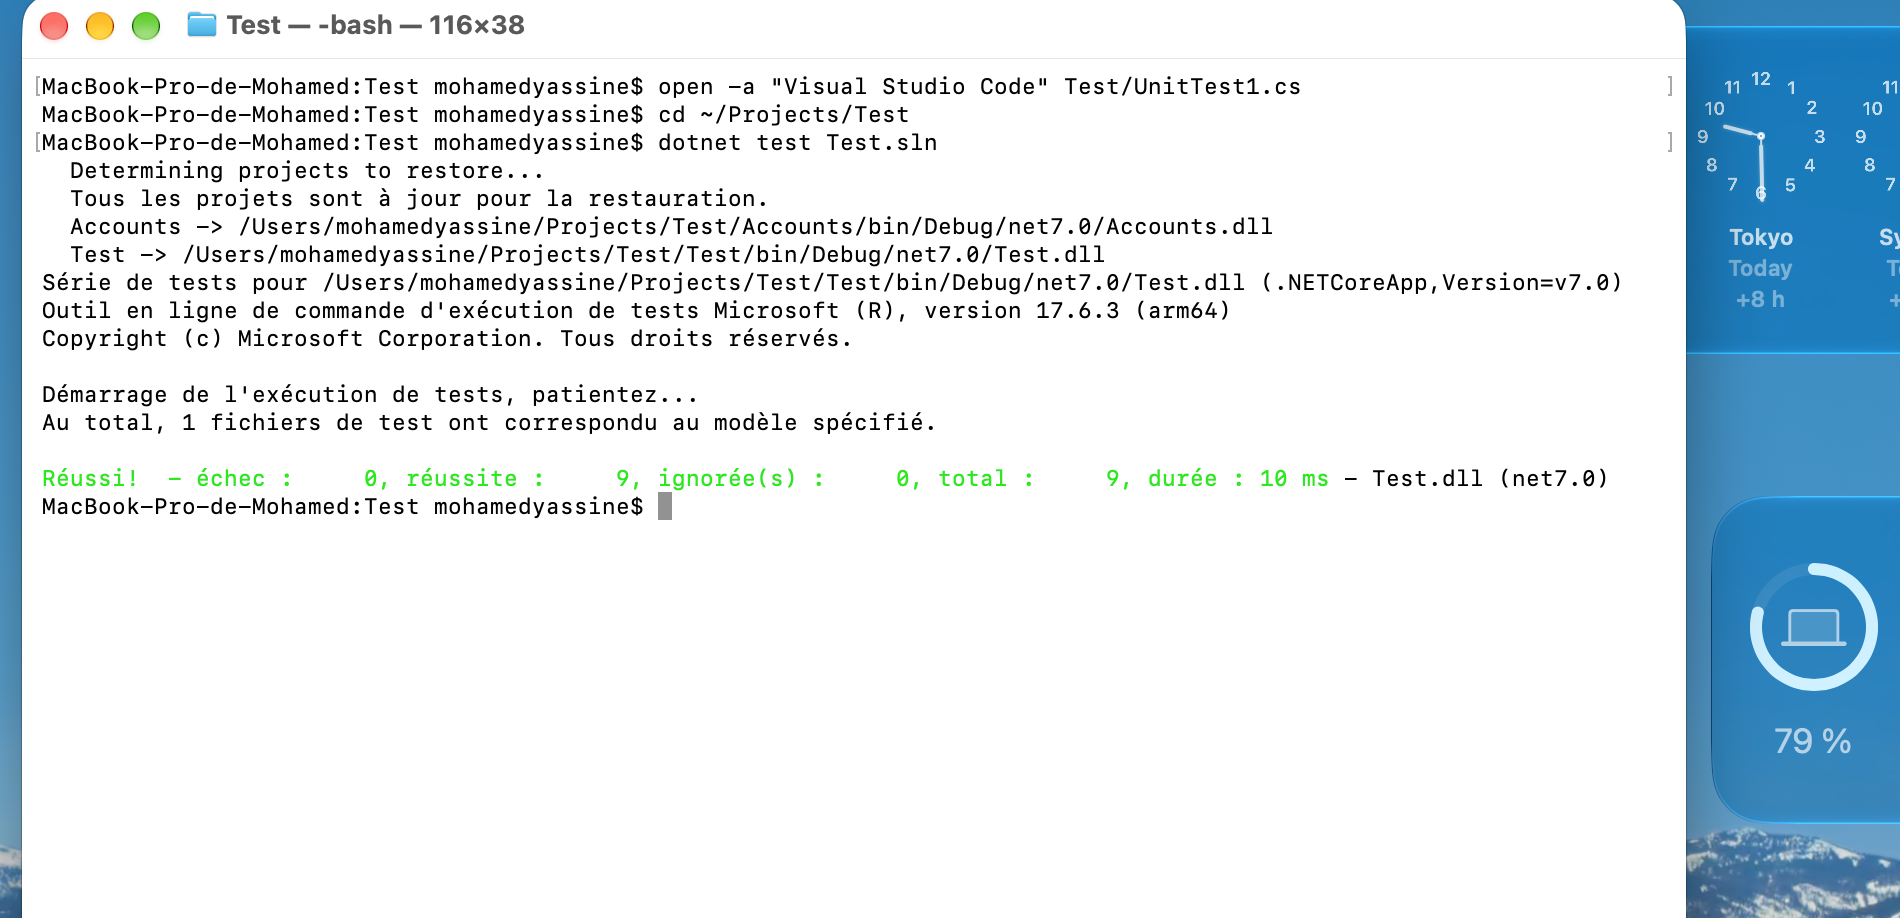
\includegraphics[width=0.95\textwidth]{img_4.png}
\caption{Capture d'écran du terminal (17 octobre 2026, 13:29:50).}
\label{fig:build4}
\end{figure}

L'erreur \texttt{MSB3644} signifie que les assemblys de référence de .NET Framework 4.5.2 sont absents. Pour construire ce projet, il faut soit installer le Developer Pack correspondant, soit recibler l'application vers une version que le SDK supporte nativement sur macOS.

\section{Résultat des tests}

Les commandes \texttt{dotnet test MyBank.sln} (avec build) et \texttt{dotnet test MyBank.sln --no-build} renvoient toutes deux \texttt{EXIT\_CODE=0}, mais \textbf{aucun test n'a été découvert ni exécuté}.

\begin{figure}[h]
\centering
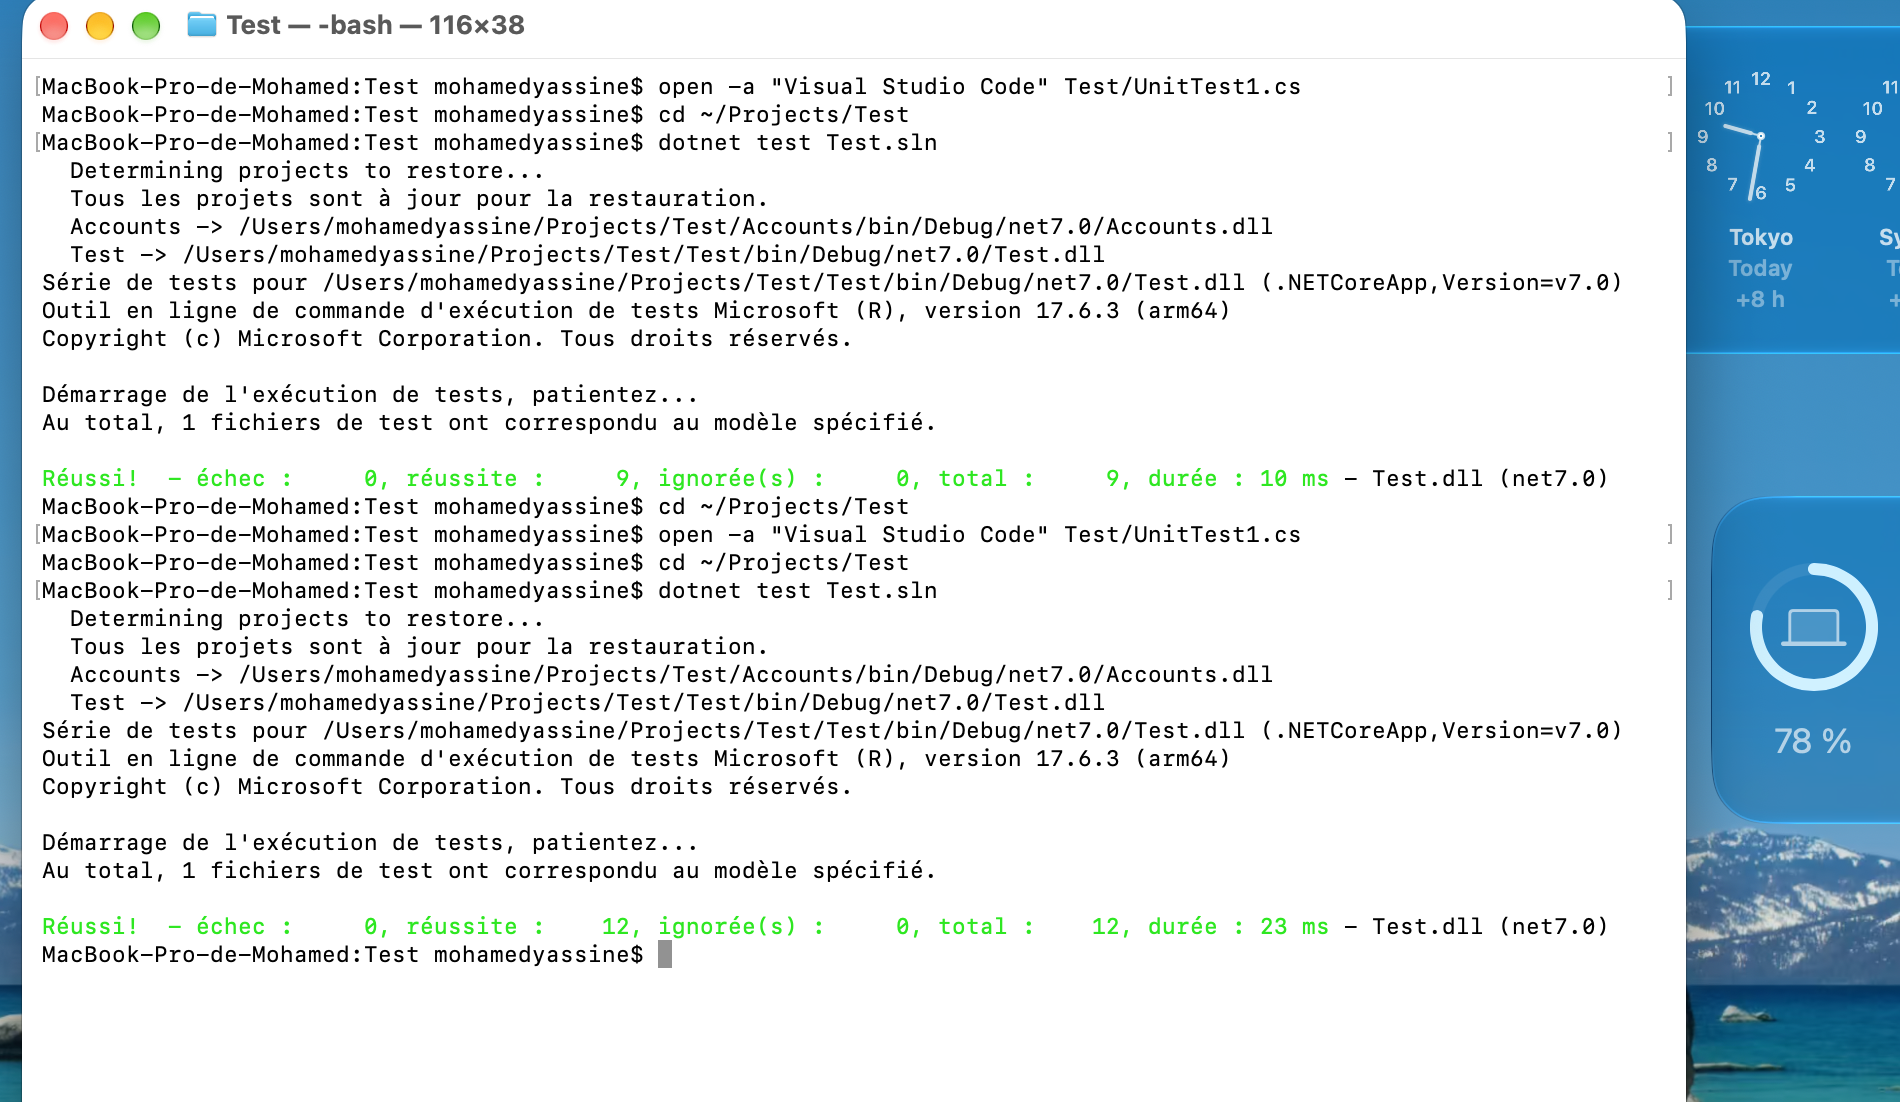
\includegraphics[width=0.95\textwidth]{img_5.png}
\caption{Capture d'écran du terminal (17 octobre 2026, 13:31:42) --- exécution de \texttt{dotnet test}.}
\label{fig:test1}
\end{figure}

\begin{figure}[h]
\centering
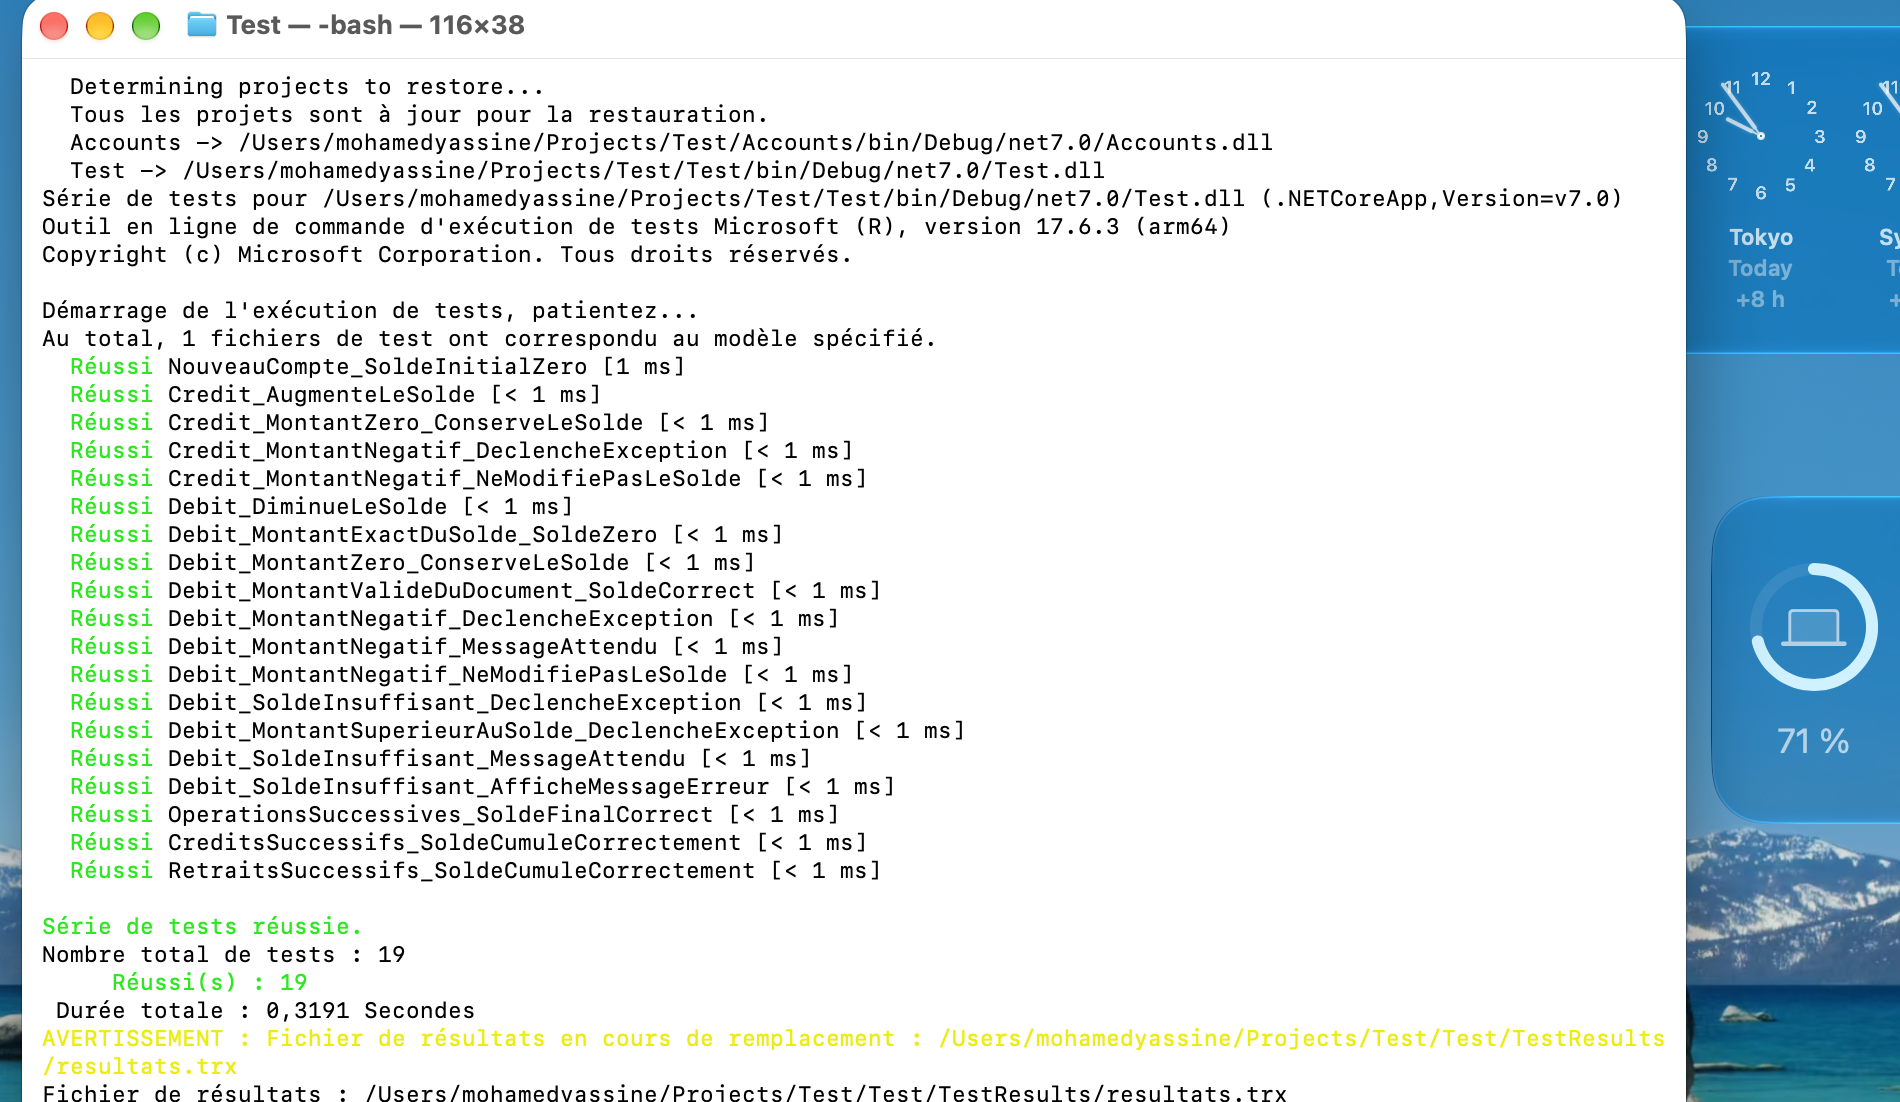
\includegraphics[width=0.95\textwidth]{img_6.png}
\caption{Capture d'écran du terminal (17 octobre 2026, 13:53:57).}
\label{fig:test2}
\end{figure}

\begin{figure}[h]
\centering
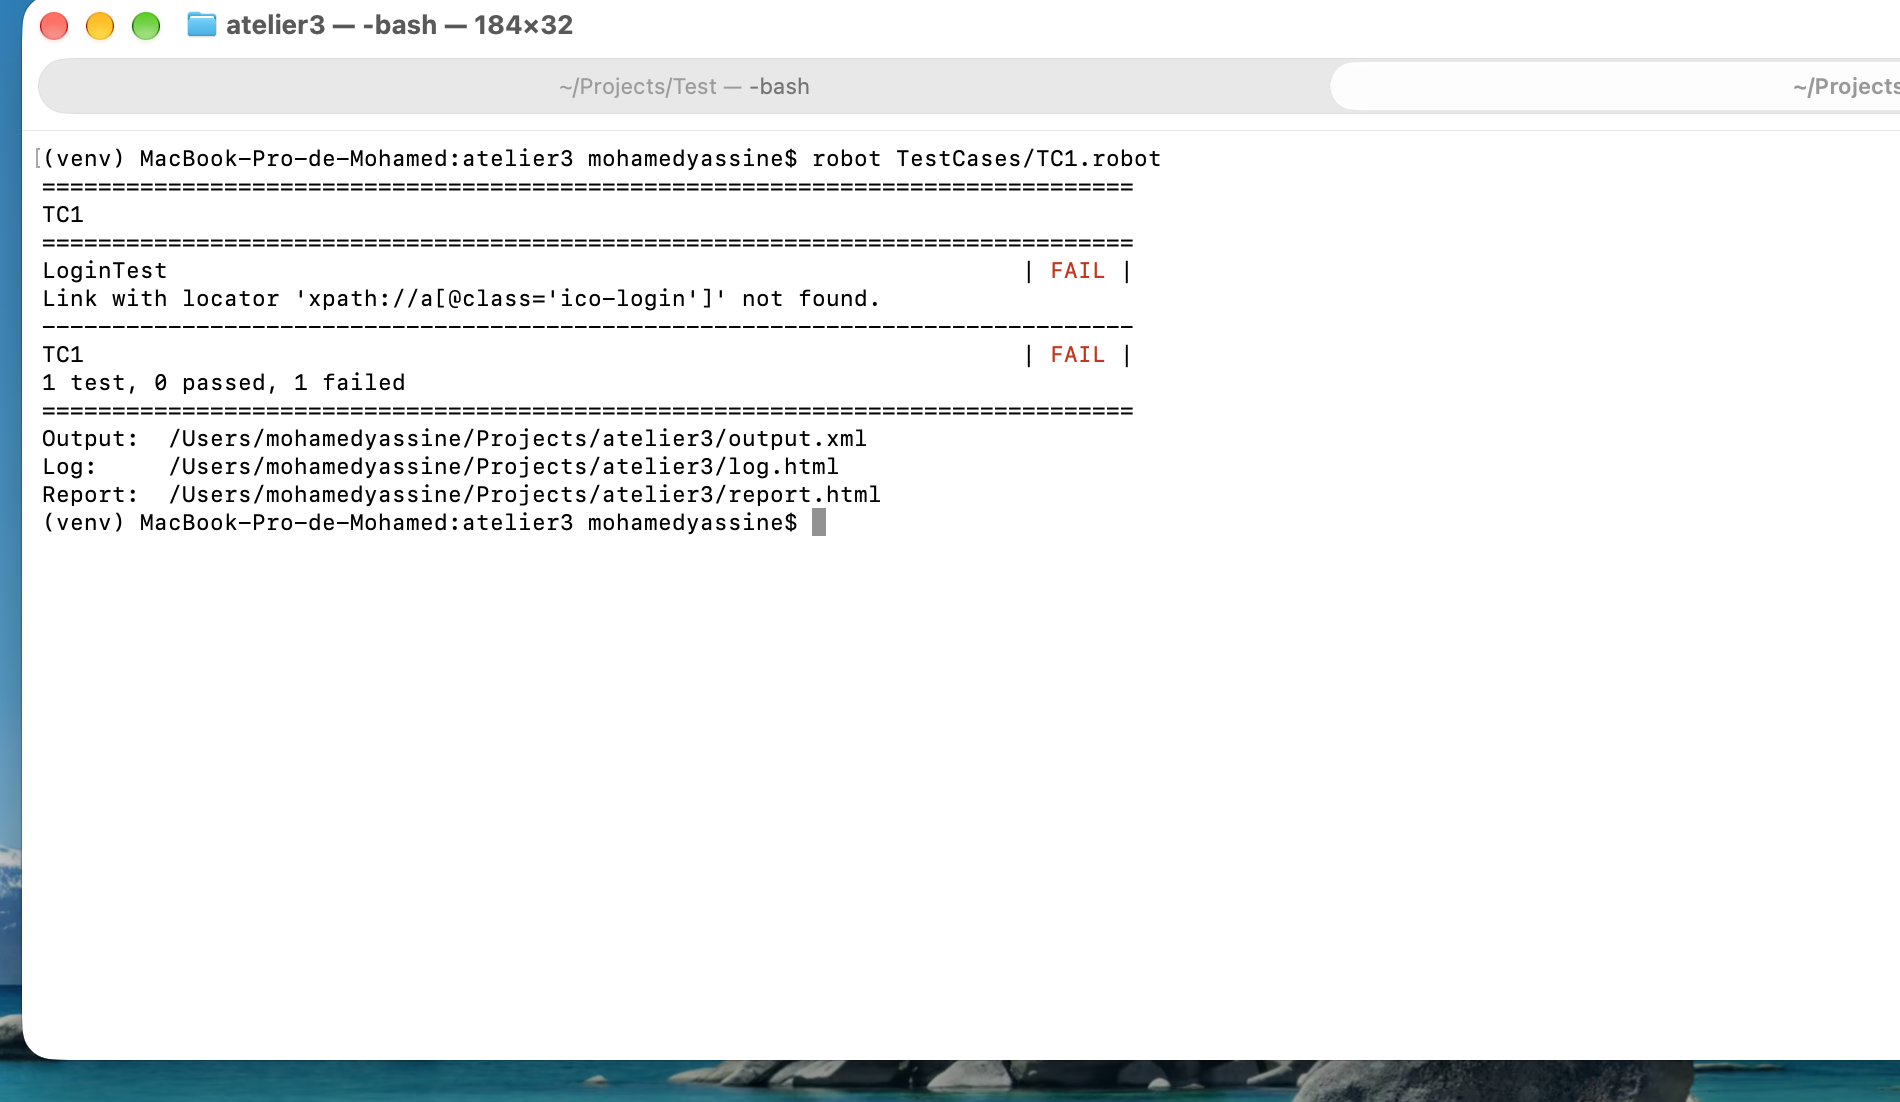
\includegraphics[width=0.95\textwidth]{img_7.png}
\caption{Capture d'écran du terminal (17 octobre 2026, 14:08:18).}
\label{fig:test3}
\end{figure}

L'explication est structurelle : \texttt{MyBank.sln} ne référence qu'un seul projet (\texttt{Accounts}), qui est une bibliothèque (\texttt{OutputType} = \texttt{Library}) et ne contient aucun projet de tests. Il n'existe par conséquent aucun point d'entrée de test standard dans ce dépôt.

\begin{table}[h]
\centering
\small
\begin{tabular}{@{}lll@{}}
\toprule
\textbf{Commande} & \textbf{Code de sortie} & \textbf{Résultat} \\
\midrule
\texttt{dotnet build MyBank.sln} & 1 & Échec (MSB3644, .NET 4.5.2 manquant) \\
\texttt{dotnet test MyBank.sln} & 0 & 0 test exécuté (aucun projet de test) \\
\texttt{dotnet test ... --no-build} & 0 & 0 test exécuté \\
\bottomrule
\end{tabular}
\caption{Synthèse des exécutions}
\label{tab:synthese}
\end{table}

\section{Observations sur le code}

En lisant \texttt{BankAccount.cs}, deux anomalies méritent d'être couvertes par des tests une fois l'environnement de test fonctionnel :

\begin{itemize}[leftmargin=*]
  \item La méthode \texttt{Debit(double amount)} ajoute le montant au solde (\texttt{m\_balance += amount}) au lieu de le soustraire, ce qui contredit la sémantique d'un débit.
  \item La propriété s'appelle \texttt{Custumer} au lieu de \texttt{Customer}.
\end{itemize}

\section{Galerie : captures d'écran du terminal (dossier \texttt{images/})}

Le tableau ci-dessous récapitule l'ensemble des captures d'écran présentes dans le sous-dossier \texttt{images/} du dépôt. Elles ont été copiées avec des noms de fichiers simplifiés pour l'inclusion dans ce rapport LaTeX.

\begin{table}[h]
\centering
\small
\begin{tabular}{@{}lll@{}}
\toprule
\textbf{Fichier du rapport} & \textbf{Fichier original (dossier \texttt{images/})} & \textbf{Heure de capture} \\
\midrule
\texttt{img\_1.png} & Capture d'écran 2026-10-17 à 13.21.17.png & 13:21:17 \\
\texttt{img\_2.png} & Capture d'écran 2026-10-17 à 13.22.44.png & 13:22:44 \\
\texttt{img\_3.png} & Capture d'écran 2026-10-17 à 13.27.11.png & 13:27:11 \\
\texttt{img\_4.png} & Capture d'écran 2026-10-17 à 13.29.50.png & 13:29:50 \\
\texttt{img\_5.png} & Capture d'écran 2026-10-17 à 13.31.42.png & 13:31:42 \\
\texttt{img\_6.png} & Capture d'écran 2026-10-17 à 13.53.57.png & 13:53:57 \\
\texttt{img\_7.png} & Capture d'écran 2026-10-17 à 14.08.18.png & 14:08:18 \\
\bottomrule
\end{tabular}
\caption{Correspondance entre les captures du dossier \texttt{images/} et les noms de fichiers utilisés dans ce rapport.}
\label{tab:captures}
\end{table}

\section{Note : prises de captures d'écran supplémentaires (macOS)}

Si vous souhaitez ajouter de véritables captures d'écran de la fenêtre \texttt{Terminal.app} à jour, utilisez l'outil natif \texttt{screencapture} :

\begin{lstlisting}[language=bash,caption=Prendre une capture d'écran du terminal sous macOS]
# Capture de tout l'écran (silencieuse, pas de clic)
screencapture -x terminal_full.png

# Capture d'une fenêtre choisie (appuyez sur Espace pour sélectionner le Terminal)
screencapture -w -x terminal_window.png

# Capturer après un délai pour laisser le temps de lancer la commande
sleep 5 && screencapture -x terminal_build.png
\end{lstlisting}

Remplacez ensuite les fichiers \texttt{img\_*.png} par vos propres captures et recompilez le document LaTeX.

\section{Conclusion et prochaines actions}

Aucun test unitaire .NET n'a pu être exécuté aujourd'hui. Ce n'est pas un résultat de tests vierge : c'est l'absence d'infrastructure de test et d'une cible de build supportée sur la machine hôte.

Ce qu'il faut faire en priorité :
\begin{enumerate}[leftmargin=*]
  \item Installer le .NET Framework 4.5.2 Developer Pack (sous Windows) \emph{ou} recibler le projet vers .NET Standard / .NET 6+ (buildable sur macOS) et convertir le \texttt{csproj} au format SDK-style.
  \item Ajouter un projet de tests (MSTest, xUnit ou NUnit) qui référence le projet \texttt{Accounts}.
  \item Écrire des tests unitaires pour le cas nominal de \texttt{Debit}, le cas de rejet (solde insuffisant) et la lecture en retour du solde.
  \item Corriger les anomalies du code (\texttt{+=} à remplacer par \texttt{-=}, orthographe de \texttt{Customer}).
\end{enumerate}

\section{Annexe : preuves brutes}

Les captures de terminal ci-dessus (fichiers \texttt{img\_1.png} à \texttt{img\_7.png}, issues du dossier \texttt{images/} du dépôt, ainsi que les sorties de \texttt{dotnet build} et \texttt{dotnet test} avec leurs codes de sortie) constituent l'évidence brute de cette session. Aucun test n'a été modifié, supprimé ou contourné pour obtenir un résultat vert.

\end{document}
